%%%%%%%%%%%%%%%%%%%%%%%%%%%%%%%%%%%%%%%%%
% FRI Data Science_report LaTeX Template
% Version 1.0 (28/1/2020)
% 
% Jure Demšar (jure.demsar@fri.uni-lj.si)
%
% Based on MicromouseSymp article template by:
% Mathias Legrand (legrand.mathias@gmail.com) 
% With extensive modifications by:
% Antonio Valente (antonio.luis.valente@gmail.com)
%
% License:
% CC BY-NC-SA 3.0 (http://creativecommons.org/licenses/by-nc-sa/3.0/)
%
%%%%%%%%%%%%%%%%%%%%%%%%%%%%%%%%%%%%%%%%%


%----------------------------------------------------------------------------------------
%	PACKAGES AND OTHER DOCUMENT CONFIGURATIONS
%----------------------------------------------------------------------------------------
\documentclass[fleqn,moreauthors,10pt]{ds_report}
\usepackage[english]{babel}

\graphicspath{{fig/}}

\usepackage[bibstyle=authoryear,maxnames=2,minnames=1]{biblatex}
\addbibresource{report.bib}


%----------------------------------------------------------------------------------------
%	ARTICLE INFORMATION
%----------------------------------------------------------------------------------------

% Header
\JournalInfo{FRI Natural language processing course 2024}

% Interim or final report
\Archive{Project report} 
%\Archive{Final report} 

% Article title
\PaperTitle{Slovenian Instruction-based Corpus Generation} 

% Authors (student competitors) and their info
\Authors{Jernej Ulčakar, Jon Kuhar, Bella Muradian}

% Advisors
\affiliation{\textit{Advisors: Slavko Žitnik}}

% Keywords
\Keywords{LLM,Slovene,Training}
\newcommand{\keywordname}{Keywords}


%----------------------------------------------------------------------------------------
%	ABSTRACT
%----------------------------------------------------------------------------------------

\Abstract{
This study explores the utilization of vast human conversation over web forums to train a multilingual fine-tune of existing large language models (LLM), efficient enough to train and run on consumer-grade hardware.
}

%----------------------------------------------------------------------------------------

\begin{document}

% Makes all text pages the same height
\flushbottom 

% Print the title and abstract box
\maketitle 

% Removes page numbering from the first page
\thispagestyle{empty} 

%----------------------------------------------------------------------------------------
%	ARTICLE CONTENTS
%----------------------------------------------------------------------------------------

\section*{Introduction}
Large Language Models (LLMs) have shown great promise as highly capable AI assistants that excel in complex reasoning tasks requiring expert knowledge across a wide range of fields, including in specialized domains such as programming and creative writing. They enable interaction with humans through intuitive chat interfaces, which has led to rapid and widespread adoption among the general public.

We fine tune a model on conversations from slovene forums such as \href{https://forum.over.net/forum/}{Med.Over.Net}, \href{www.slo-tech.com}{slo-tech} and \href{https://www.reddit.com/r/Slovenia/}{Reddit Slovenia}. We collected this data using WinHTTracker scraper and python for parsing.

For the base model we used \href{https://github.com/tloen/alpaca-lora}{Alpaca-lora}, the \emph{low-rank adaptation} (LoRA)\cite{hu2021lowrank} of the Alpaca\cite{Bommasani2021FoundationModels} model. This model is itself a fine-tune of the Llama\cite{touvron2023llama} model. It is fine-tuned with a large set of conversations and was relatively cheap to make. The LoRA version is even more concise, allowing for very cheap further training, doable on consumer hardware.
The model should have a basic understanding of the slovenian language because Llama's training dataset contains 4.5\% wikipedia dumps from June-August 2022. These dumps cover 20 languages, including slovenian.

We published the code and the model weights on \href{https://github.com/UL-FRI-NLP-2023-2024/ul-fri-nlp-course-project-tree-pipit/}{github}.

%Your task is to get to know LLMs and try to understand their creation from higher levels. Try to prepare large amounts of conversational data in Slovene (this is the focus of this task!) that is correctly organized and of good quality to be fed into fine-tuning a multi-lingual LLM (that supports Slovene). Demonstrate work by adapting a model to fine-tune a conversational agent for Slovene.

%	These latex files are intended to serve as a the template for the NLP course at FRI.  The template is adapted from the FRI Data Science Project Competition. template  If you find mistakes in the template or have problems using it, please consult Jure Demšar (\href{mailto:jure.demsar@fri.uni-lj.si}{jure.demsar@fri.uni-lj.si}).
	
%	In the Introduction section you should write about the relevance of your work (what is the purpose of the project, what will we solve) and about related work (what solutions for the problem already exist). Where appropriate, reference scientific work conducted by other researchers. For example, the work done by Demšar et al. \cite{Demsar2016BalancedMixture} is very important for our project. The abbreviation et al. is for et alia, which in latin means and others, we use this abbreviation when there are more than two authors of the work we are citing. If there are two authors (or if there is a single author) we just write down their surnames. For example, the work done by Demšar and Lebar Bajec \cite{Demsar2017LinguisticEvolution} is also important for successful completion of our project.


%------------------------------------------------

\section*{Related Works}

\noindent
\textbf{Llama 2} (2023) \cite{touvron2023llama} is a collection of pretrained and fine-tuned
large language models (LLMs) ranging in scale from 7 billion to 70 billion parameters.
They introduced LLMs that are fine-tuned, called Llama 2-Chat, and are optimized for dialogue use cases.

\noindent
\textbf{BLOOM} (2023) \cite{workshop2023bloom} is a collection of pretrained and fine-tuned
A 176B-parameter open-access language model designed and built thanks to a collaboration of hundreds of researchers. BLOOM is a decoder-only Transformer language model that was trained on the ROOTS corpus \cite{laurençon2023bigscience}, a dataset comprising hundreds of
sources in 46 natural and 13 programming languages (59 in total). BLOOM achieves competitive performance on a wide variety of benchmarks, with stronger results after undergoing multitask prompted fine-tuning. To facilitate future research and applications using LLMs.

\noindent
\textbf{Training models} (2022) \cite{Ouyang2022TrainingLM} this paper contains instructions in how to fine-tune language models with user intent on a wide range of tasks by using human feedback.
Starting with a set of labeler-written prompts and prompts
submitted through the OpenAI API, they collected a dataset of labeler demonstrations
of the desired model behavior, which they later used to fine-tune GPT-3 using supervised
learning and the collect the dataset of rankings of model outputs. These are used to further fine-tune the model using reinforcement learning from human feedback. The model names are InstructGPT. In human evaluations on
our prompt distribution, outputs from the 1.3B parameter InstructGPT model are
preferred to outputs from the 175B GPT-3, despite having 100x fewer parameters.
Moreover, InstructGPT models show improvements in truthfulness and reductions
in toxic output generation while having minimal performance regressions on public
NLP datasets. Even though InstructGPT still makes simple mistakes, their results
show that fine-tuning with human feedback is a promising direction for aligning
language models with human intent.

%------------------------------------------------

\section*{Methods}

\subsection*{Scraping}

We used WinHTTrack, a powerful web scraping tool, to scrape data from three online forums: Med.Over.Net, slo-tech.com and forum.over.net.

We configured WinHTTrack to navigate through the forum websites systematically, crawling through the existing links to access all posts and comments.

Each website contains more than just discussions with comments, for example user pages, about info, links to outside of the page. To ensure efficient parsing, we needed to analize the structure of each forum's urls to make sure only the urls corresponding to forum threads are crawled. An example of the process for the site slotech.com is in \ref{sssection:sloforum}.

We made sure to respect the forums' \texttt{robots.txt}. This is done automatically by WinHTTrack and actually simplified the process as all the rulesets prevented scraping of data we didn't want to scrape anyway.

\subsubsection*{Scraping slo\-tech.com forums}\label{sssection:sloforum}

Slo-tech is the biggest slovenian computer forum that has existed for over two decades. On the front page of the forum we see the split into many subforums in the format of \texttt{/forum/\{id\}}. The subforums are not listed in increasing order and not all ids are taken. The lowest id forum is ''Zvok in slika", \texttt{/forum/4}. There are two special subforums that are not scraped as they link to threads in other subforums, ''Teme zadnjih 24 ur" (Threads made in the last 24 hours) and ''Neodgovorjene teme" (Threads without responses).

The next pages on the forum are accessed with \\ \texttt{/forum/\{id\}/1}, \texttt{/forum/\{id\}/2} and so on. \\ \texttt{/forum/\{id\}/0} is also theoretically valid for the access of the first page but this is not used inside of the pages for the scraper to pick up.

The threads have url structure \texttt{/forum/t\{id\}}. They contain up to 50 messages. Next pages are accessed with \texttt{/forum/t\{id\}/\{n\}}. $n$ represents the number of the next message shown so page 2 is \texttt{/49}, page 3 is \texttt{/99} and so on. For large pages the navigation includes \texttt{/konec} to jump to the last page. The first page is linked to as \texttt{/0}. We set up the scraper to ignore the \texttt{/0} and \texttt{/konec} as they lead to duplicated pages.

At the bottom of threads there is usually a table of related posts. These do not necessarily link to the same subforum This is a bit of a problem if we want to be selective about scraping a specific subforum. There is no info in the url of a thread to indicate the subforum it is in.

The robots.txt of slo-tech permits accessing all forum pages but not user pages \texttt{/profili} and the lists of user threads \texttt{/u\{id\}}, user comments \texttt{/c\{id\}} and threads contributed to by a user \texttt{/s\{id\}}. This is fine for us as we do not need to scrape user profiles.

Important parameters used for the scraper, the initial urls and scan rules, are available in the github repository in the \texttt{scripts/scraping} directory.

\subsection*{Parsing data}

Similarly to scraping, each forum had a different structure in the html. To parse this structure we developed parsers in python using the \texttt{BeautifulSoup} library. We use this on each thread to extract the users, dates, content and quoted content. Not all of this data is going to be used, but it was still collected for completeness. The threads are collected into a json file. The code used for parsing is available in the \texttt{scripts/parsing} directory and the parsed files are in \texttt{results/parsing}.

\subsection*{Generating instructions}

The original training of the Alpaca model was done by fine-tuning on a list of 52k data points in the format of:

\lstset{language=Python}
\lstset{label={lst:code_direct}}
\begin{lstlisting}
{
    "instruction": "...",
    "input": "...",
    "output": "..."
}
\end{lstlisting}

Our fine-tuning script will also use this format to keep the original training script with minimal modifications.

Because many threads start with a question, we decided to format our instruction set such that the title and original posts are combined as the instruction. Because many of the first responses directly address and answer the question we use these as the output.

The code used for transforming our parsed data into this format is in \texttt{scripts/generate}, the instruction set is in \texttt{results/generate}.

\subsection*{Training}

The training script was only slightly modified from the original Alpaca-lora's training script. Since we wanted to keep the lora focused on instruction responses, the initial weights were set to those from Alpaca-lora. We used the following hyperparameters:
\begin{center}
batch\_size=128,
micro\_batch\_size=4,
num\_epochs=3,
learning\_rate=0.0003,
cutoff\_len=256,
val\_set\_size=2000,
lora\_r=8,
lora\_alpha=16,
lora\_dropout=0.05
\end{center}

\subsection*{Evaluation}

We used the human evaluation instructions from Self-instruct\ref{}, translating a small set to slovene and evaluating it.

\iffalse
Use the Methods section to describe what you did an how you did it -- in what way did you prepare the data, what algorithms did you use, how did you test various solutions ... Provide all the required details for a reproduction of your work.

Below are \LaTeX examples of some common elements that you will probably need when writing your report (e.g. figures, equations, lists, code examples ...).


\subsection*{Equations}

You can write equations inline, e.g. $\cos\pi=-1$, $E = m \cdot c^2$ and $\alpha$, or you can include them as separate objects. The Bayes’s rule is stated mathematically as:

\begin{equation}
	P(A|B) = \frac{P(B|A)P(A)}{P(B)},
	\label{eq:bayes}
\end{equation}

where $A$ and $B$ are some events. You can also reference it -- the equation \ref{eq:bayes} describes the Bayes's rule.

\subsection*{Lists}

We can insert numbered and bullet lists:

% the [noitemsep] option makes the list more compact
\begin{enumerate}[noitemsep] 
	\item First item in the list.
	\item Second item in the list.
	\item Third item in the list.
\end{enumerate}

\begin{itemize}[noitemsep] 
	\item First item in the list.
	\item Second item in the list.
	\item Third item in the list.
\end{itemize}

We can use the description environment to define or describe key terms and phrases.

\begin{description}
	\item[Word] What is a word?.
	\item[Concept] What is a concept?
	\item[Idea] What is an idea?
\end{description}


\subsection*{Random text}

This text is inserted only to make this template look more like a proper report. Lorem ipsum dolor sit amet, consectetur adipiscing elit. Etiam blandit dictum facilisis. Lorem ipsum dolor sit amet, consectetur adipiscing elit. Interdum et malesuada fames ac ante ipsum primis in faucibus. Etiam convallis tellus velit, quis ornare ipsum aliquam id. Maecenas tempus mauris sit amet libero elementum eleifend. Nulla nunc orci, consectetur non consequat ac, consequat non nisl. Aenean vitae dui nec ex fringilla malesuada. Proin elit libero, faucibus eget neque quis, condimentum laoreet urna. Etiam at nunc quis felis pulvinar dignissim. Phasellus turpis turpis, vestibulum eget imperdiet in, molestie eget neque. Curabitur quis ante sed nunc varius dictum non quis nisl. Donec nec lobortis velit. Ut cursus, libero efficitur dictum imperdiet, odio mi fermentum dui, id vulputate metus velit sit amet risus. Nulla vel volutpat elit. Mauris ex erat, pulvinar ac accumsan sit amet, ultrices sit amet turpis.

Phasellus in ligula nunc. Vivamus sem lorem, malesuada sed pretium quis, varius convallis lectus. Quisque in risus nec lectus lobortis gravida non a sem. Quisque et vestibulum sem, vel mollis dolor. Nullam ante ex, scelerisque ac efficitur vel, rhoncus quis lectus. Pellentesque scelerisque efficitur purus in faucibus. Maecenas vestibulum vulputate nisl sed vestibulum. Nullam varius turpis in hendrerit posuere.

\subsection*{Figures}

You can insert figures that span over the whole page, or over just a single column. The first one, \figurename~\ref{fig:column}, is an example of a figure that spans only across one of the two columns in the report.

\begin{figure}[ht]\centering
	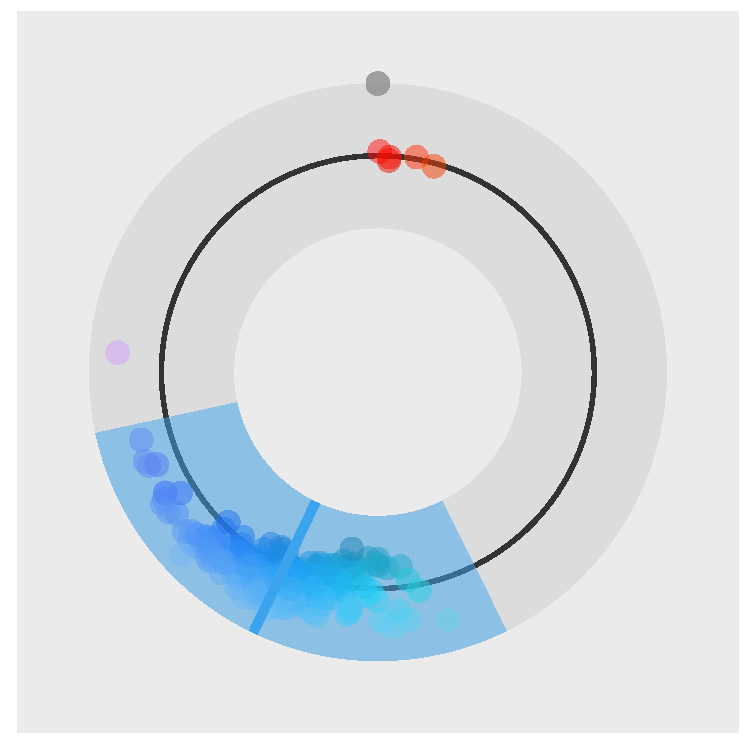
\includegraphics[width=\linewidth]{single_column.pdf}
	\caption{\textbf{A random visualization.} This is an example of a figure that spans only across one of the two columns.}
	\label{fig:column}
\end{figure}

On the other hand, \figurename~\ref{fig:whole} is an example of a figure that spans across the whole page (across both columns) of the report.

% \begin{figure*} makes the figure take up the entire width of the page
\begin{figure*}[ht]\centering 
	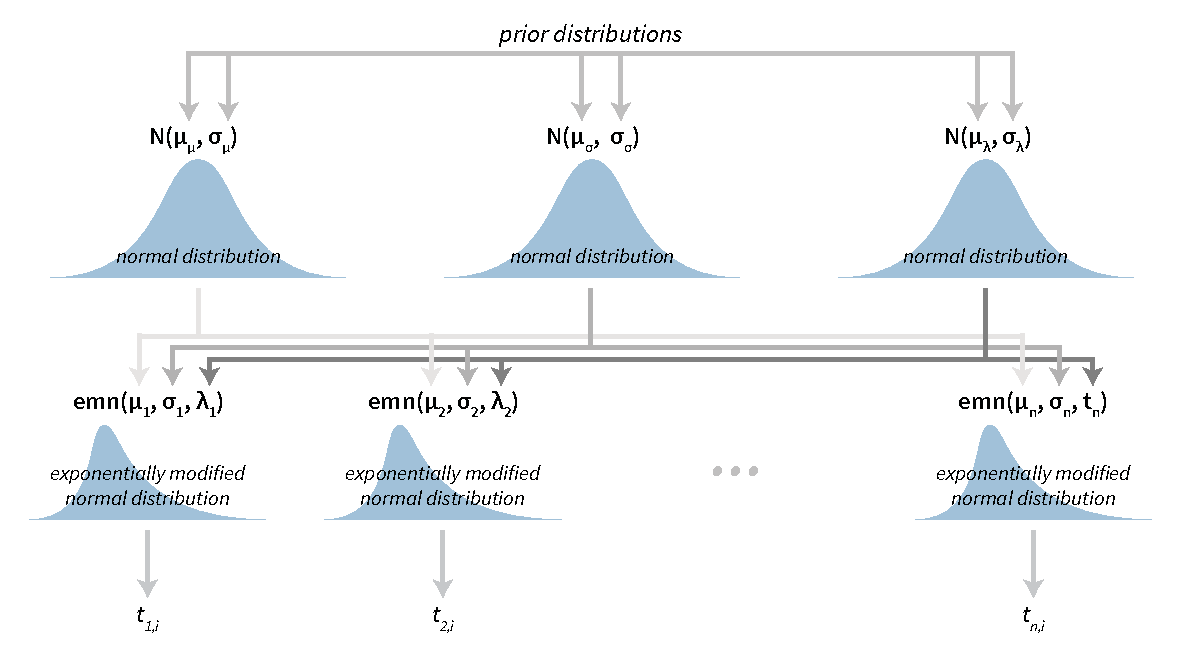
\includegraphics[width=\linewidth]{whole_page.pdf}
	\caption{\textbf{Visualization of a Bayesian hierarchical model.} This is an example of a figure that spans the whole width of the report.}
	\label{fig:whole}
\end{figure*}


\subsection*{Tables}

Use the table environment to insert tables.

\begin{table}[hbt]
	\caption{Table of grades.}
	\centering
	\begin{tabular}{l l | r}
		\toprule
		\multicolumn{2}{c}{Name} \\
		\cmidrule(r){1-2}
		First name & Last Name & Grade \\
		\midrule
		John & Doe & $7.5$ \\
		Jane & Doe & $10$ \\
		Mike & Smith & $8$ \\
		\bottomrule
	\end{tabular}
	\label{tab:label}
\end{table}


\subsection*{Code examples}

You can also insert short code examples. You can specify them manually, or insert a whole file with code. Please avoid inserting long code snippets, advisors will have access to your repositories and can take a look at your code there. If necessary, you can use this technique to insert code (or pseudo code) of short algorithms that are crucial for the understanding of the manuscript.

\lstset{language=Python}
\lstset{caption={Insert code directly from a file.}}
\lstset{label={lst:code_file}}
\lstinputlisting[language=Python]{code/example.py}

\lstset{language=R}
\lstset{caption={Write the code you want to insert.}}
\lstset{label={lst:code_direct}}
\begin{lstlisting}
import(dplyr)
import(ggplot)

ggplot(diamonds,
	   aes(x=carat, y=price, color=cut)) +
  geom_point() +
  geom_smooth()
\end{lstlisting}

%------------------------------------------------
\fi
\section*{Results}
The scraping statistics are in table~\ref{}. We expected to get rate limited but that only happened late when enough threads were already scraped.

The results of data parsing are in table~\ref{}. The data was parsed well. The only junk remaining was inside the posted content of each user as well as the users type of speech (this includes typos and accent-like typing). Generating instructions was also without issues.

The training was done on \href{https://cloud.vast.ai/create/}{vast.ai}. The GPU we used was an RTX 6000Ada with 81.4 TFlops and 48GB of VRAM. The VRAM was underutilized, only using up to 10GB while training. This means we could have used a less performant GPU without running out of memory.

In total, training took 3h for 300 iterations.

\iffalse
Use the results section to present the final results of your work. Present the results in a objective and scientific fashion. Use visualisations to convey your results in a clear and efficient manner. When comparing results between various techniques use appropriate statistical methodology.
\fi


%------------------------------------------------

\section*{Discussion}

Use the Discussion section to objectively evaluate your work, do not just put praise on everything you did, be critical and exposes flaws and weaknesses of your solution. You can also explain what you would do differently if you would be able to start again and what upgrades could be done on the project in the future.


%------------------------------------------------
\iffalse
\section*{Acknowledgments}

Here you can thank other persons (advisors, colleagues ...) that contributed to the successful completion of your project.
\fi

%----------------------------------------------------------------------------------------
%	REFERENCE LIST
%----------------------------------------------------------------------------------------
\printbibliography
%\bibliographystyle{unsrt}
%\bibliography{report}


\end{document}
